\documentclass{article}
\usepackage[utf8]{inputenc}
\usepackage{amsmath}
\usepackage{xfrac}
\usepackage[utf8]{inputenc}
\usepackage[english]{babel}
\usepackage{graphicx}
\usepackage{subcaption}
\usepackage{csquotes}
\usepackage{biblatex}
\usepackage[colorlinks=true]{hyperref}
\usepackage{siunitx}
\usepackage{wrapfig}
\usepackage{media9}
\usepackage{multirow}
\usepackage{graphbox}

\addbibresource{references.bib}
\graphicspath{ {./images/} }
\addmediapath{ {./images/animations/} }
\makeatletter
\def\input@path{{./figures/}}
\makeatother

\title{Time-varying frequency Estimation of narrow-band signals via Extended Kalman Filter and Unscented Kalman Filter}
\author{Emanuele Dalla Longa \and Sergio Gandola}
\date{September 2018}

\begin{document}

\maketitle

\begin{abstract}
In this paper the problem of estimating the frequency of a narrow-band harmonic signal embedded in noise is discussed; in particular, Kalman filter-based approaches such as the \emph{Extendend Kalman Filter} (EKF) and the \emph{Unscented Kalman Filter} (UKF). In order to evaluate the achieved estimation quality of the algorithms, two criteria  are introduced: the \emph{Performance Index} (PI) and the \emph{Robustness Index} (RI), plus an auxiliary \emph{Convergence Ratio}. Tests have been performed both on recorded real world signals and on generated noisy signals.
\end{abstract}

\section{Introduction}
This work explores and compares the capabilities of Kalman filter-based frequency tracking methods such the \emph{Extendend Kalman Filter} (EKF) and the \emph{Unscented Kalman Filter} (UKF) to track the time-varying frequency of a narrow-band harmonic signal. These results are compared with those by \citeauthor{UKF} in \cite{UKF}. 

In order to evaluate the achieved estimation quality of the algorithms, two criteria are used: the \emph{Performance Index} (PI) and the \emph{Robustness Index} (RI), described in\cite{UKF}. An auxiliary \emph{Convergence Ratio} is introduced to better interpret the PI plots.

Two signals are considered: a single frequency sinusoidal signal recorded from the real world and a generated noisy signal with time-varying frequency following a step profile. The algorithm was able to estimate the real world signal with accuracies $\sim 10^{-7}$ and achieve performances consistent with \cite{UKF}.

In the last section the obtained results are shown and discussed, with emphasis on some behaviors which may be due to numerical errors.

\section{Previous works}
This work builds on \cite{EKF} for the EKF implementation and on \cite{UKF} for the performance evaluation. \cite{UKF} was also used along with \cite{ukftutorial} for the implementation of the UKF algorithm.

\section{Problem statement}
Consider the signal : 
$$y(t) = s(t) + n(t)$$
where $n(t)$ is a broadband noise (e.g., a white noise) and $s(t)$ a sinusoid of the type $$s(t) = A\cdot\sin\big(\Phi(t) + \phi\big)$$ where $\Phi(t)$ is the instantaneous frequency as described in \cite{IF}.

The proposed model is constructed from the representation of the signal as a rotating vector in the Cartesian plane with angular velocity $\Phi(t)$. A third-order state space model (ARMA representation) is derived by taking the two projections of the vector along the axes and the instantaneous frequency as state variables: 

\[
\left\{
\begin{aligned}
x_1(t+1) &= cos(x_3(t))x_1(t)-sin(x_3(t))x_2(t) \\
x_2(t+1) &= sin(x_3(t))x_1(t)+cos(x_3(t))x_2(t) \\
x_3(t+1) &= x_3(t)+w(t) \\
y(t)  &= x_1(t)+v(t)
\end{aligned} \right.
\]

Two uncorrelated, zero mean noises $w(t)\sim WN(0,q)$ and $v(t)\sim WN(0,r)$ have been introduced, where $q$ represent the a-priori variance attributed to the state variables, while $r$ is the a-priori variance attributed to the measurement variable. As proven in \cite{EKF}, the ratio $\sigma = \sfrac{r}{q}$ alone governs the estimation performances for the EKF, and the reasoning can be extended to the UKF. This parameter regulates the trade-off between convergence quality (high sigma, low state estimation variance)  and convergence speed (ability to react quickly to abrupt frequency variations). 

We found this to be true experimentally; however, in the last section we show how and when the absolute values of the parameters $q$ and $r$ start to play a relevant role in the algorithm performances with the standard implementation.

\section{Proposed approaches}
The two approaches used in this paper are the EKF and the UKF. A brief description of the latter is given below.

\subsection{Unscented Kalman Filter}
\begin{figure}
\centering
\begin{subfigure}{0.45\textwidth}
\includemedia[width=\textwidth,activate=onclick,addresource=images/animations/ukf.mp4,flashvars={source=images/animations/ukf.mp4&autoPlay=true&loop=true}]{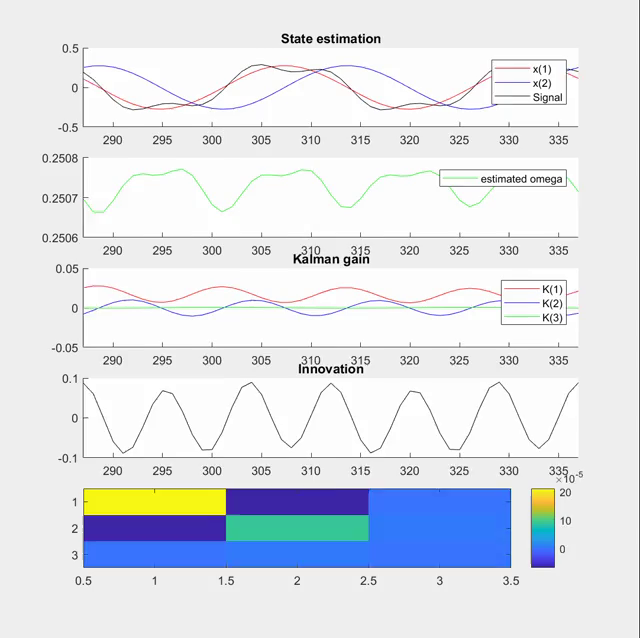
\includegraphics[width=\textwidth]{images/animations/ukf.png}}{VPlayer.swf}
\caption{Signal, estimation, Kalman gain and covariance matrix P\footnotemark.
$\omega_{\text{true}} = 0.25076 \ \sfrac{\text{rad}}{\text{sample}}$ (1760 \si{\hertz})}
\label{fig:ukf_estimation}
\end{subfigure}
\quad
\begin{subfigure}{0.4\textwidth}
\includemedia[width=\textwidth,activate=onclick,addresource=images/animations/sp.mp4,flashvars={source=images/animations/sp.mp4&autoPlay=true&loop=true}]{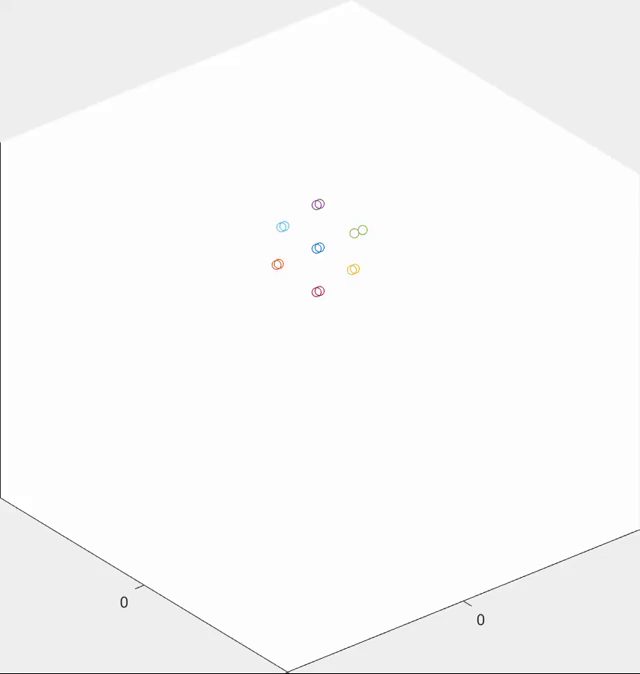
\includegraphics[width=\textwidth]{images/animations/sp.png}}{VPlayer.swf}
\caption{Evolution of sigma points in the state space}
\label{fig:ukf_sigmapoints}
\end{subfigure}

\caption{UKF visualizations}
\label{fig:ukf_visualizations}
\end{figure}
\footnotetext{It is interesting to notice how the absolute values of the elements of P are proportional to the slope of the component in the figure: higher rate of change means higher estimation variance.}
The Unscented Kalman Filter (UKF) is a widely used method to estimate the state vector of a non-linear process, based on the Unscented Transformation, which is a method for calculating the statistics of a random variable which undergoes a nonlinear transformation. It is founded on the intuition that it is easier to approximate a probability distribution than it is to approximate an arbitrary nonlinear function or transformation. 

\paragraph{Unscented transformation} The sigma points $\varsigma$ are chosen so that their mean and covariance are exactly $\hat{x}_{k-1}$ and $P_{k-1}$, where $\hat{x}_{k-1}$ is the predicted state vector and $P_{k-1}$ the covariance matrix at the previous instant. Each sigma point is then propagated through the nonlinearity, yielding in the end a cloud of transformed points. The newly estimated mean and covariance are then computed using their statistics, weighted with an optimal set of weights.

\paragraph{Data assimilation step} The Kalman gain is computed as 
$$K_k = \mathrm{Cov}(\varsigma^s_k,\varsigma^m_k) \cdot \mathrm{Cov}(\varsigma^m_k,\varsigma^m_k)^{-1}  $$
where $\varsigma^s_k$ are the sigma points propagated through the state model function and $\varsigma^m_k$ are the sigma points propagated through the measurement model function. A visualization of this is given in Figure~\ref{fig:ukf_sigmapoints}.

Then, the new state estimation is computed as:
$$\hat{x}_k = \hat{x}^s_{k|k-1} + K_k\cdot\left[y_k - \hat{x}^m_{k|k-1}\right]$$
We add to the estimate of the state vector $\hat{x}^s_{k|k-1}$, weighted mean of $\varsigma^s_{k}$, the innovation, computed as the difference between the measurement $y_k$ and the weighted mean of $\varsigma^m_k$, tuned by the Kalman gain $K_k$.

\subsection{Performance evaluation}
In order to evaluate the analysis, two different performance indices are introduced: the Performance Index (PI) and the Robustness Index (RI). As shown in the following sections, the two indices give us a metric that can be extended to every frequency tracker: they are indeed related to the capability of the tracker to attain low error at steady state, and the capability to converge, possibly rapidly, after a sudden change of the signal frequency.

\begin{figure}
    \begin{subfigure}{0.45\linewidth}
    \centering
    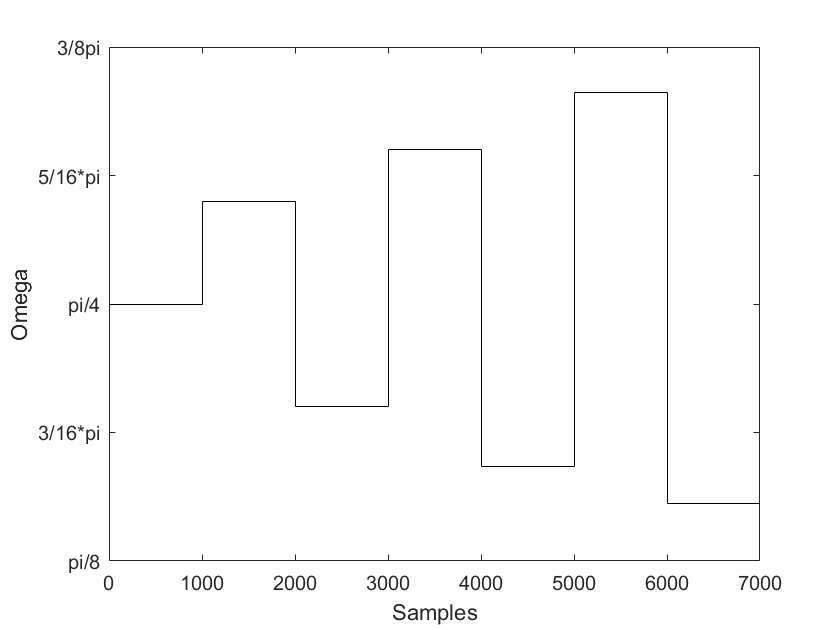
\includegraphics[width=\textwidth]{images/profiles/profile_pi.png}
    \caption{PI profile}
    \label{fig:profile_pi}
    \end{subfigure}
    \begin{subfigure}{0.45\linewidth}
    \centering
    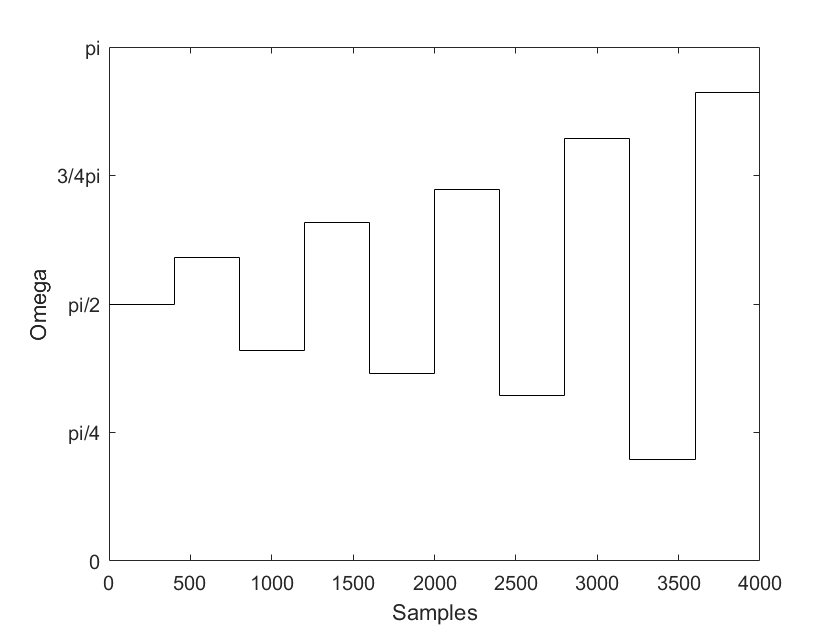
\includegraphics[width=\textwidth]{images/profiles/profile_ri.png}
    \caption{RI profile}
    \label{fig:profile_ri}
    \end{subfigure}
    \caption{Test signal frequency profile for PI and RI}
    \label{fig:profiles}
\end{figure}

\subsubsection{Performance Index}
The goal of the Performance Index is to characterize the
trade-off between the algorithm convergence rate and the error at steady-state. We can define two different intervals :
\begin{description}
    \item[Transient Interval ($T_t$)] related to the error during transient conditions
    \item[Steady State Interval ($T_{ss}$)] related to the error at steady state
\end{description}
The length of $T_t(i)$ and $T_{ss}(i)$ are different for each $i$\textsuperscript{th} step, in order to take into account the speed of convergence (the higher the step, the slower the convergence). The duration of these time steps are taken from \cite[Table~1]{UKF}.
Given $\hat{\omega}(t)$, the estimated instantaneous frequency at time $t$, it is possible to compute the $MSE$ of the estimated signal with the formula below:

\begin{equation}\label{mse}
MSE\big(e(t)\big) = MSE\big(\omega(t) - \hat{\omega}(t) \big) = \sum_{t=1}^{N}\big(\omega(t)- \hat{\omega}(t)\big)^{2}
\end{equation}

Where $N$ is the number of samples. For each $i$\textsuperscript{th} step we can define two separate errors, the transient error $e_{t,i}$ and the steady state error $e_{ss,i}$. Each error is computed within the corresponding portion of time interval of the step. We then compute $MSE(e_{t,i})$ and $MSE(e_{ss,i})$ as defined in (\ref{mse}). Then, the PI is computed as the tuple 
$$\left\{
\frac{1}{N_{\text{step}}}
\sum_{i=0}^{N_{\text{step}}}
{MSE(e_{t,i})} \ , \ 
\frac{1}{N_{\text{step}}}
\sum_{i=0}^{N_{\text{step}}}
{MSE(e_{ss,i})} 
\right\}$$ 

\subsubsection{Robustness Index}
The purpose of the Robustness Index is to evaluate the capability of the estimation method to converge after large variations of the the signal frequency. Given a frequency profile (which for this article will be the one described in Figure \ref{fig:profile_ri}), the RI is defined as a vector of length $n$, where $n$ is the number of steps in the profile. Each element $RI_i$ of the vector is the number of times the algorithm converged until step $i$, then diverged. The convergence is determined by heuristic thresholding of the MSE.

\subsubsection{Convergence ratio}
This is a novel performance metric introduced in this paper, to preserve the information about the non-converged iterations which are filtered in the plot of the PI. It is an approximation of the pointwise ratio $\frac{\text{Converged Iterations}}{\text{All Iterations}}$ of the algorithm as a function of $\sigma$. First, a boolean vector $$c^b \mid c^b_i = 1 \impliedby \text{the algorithm converged with } \sigma_i$$ is introduced. Let $c^{\text{cum}}$ be the cumulative sum of $c^b$ and $g$ a gaussian kernel. We have $$c^{\text{cum}} * \nabla g \approx \frac{dc^{\text{cum}}}{d\sigma}$$ where $\frac{dc^{\text{cum}}}{d\sigma}$ is proportional to the convergence ratio.

\section{Experiment setup}
\subsection{Signal generation}
\subsubsection{Real signal}
\begin{table}

\begin{subtable}[t]{\linewidth}
\centering
\begin{tabular}{l|c|c|c}
    & q             & $\sigma$      & MSE           \\
\hline
EKF & \num{1e-11}   & \num{1e+8}    & \num{3.60e-7} \\
\hline
UKF & \num{1e-11}   & \num{1e+8}    & \num{4.53e-7} \\
\end{tabular}
\caption{440 Hz}
\end{subtable}

\quad

\begin{subtable}{\linewidth}
\centering
\begin{tabular}{l|c|c|c}
    & q             & $\sigma$      & MSE           \\
\hline
EKF & \num{1e-11}   & \num{1e+9}    & \num{4.29e-7} \\
\hline
UKF & \num{1e-11}   & \num{1e+9}    & \num{4.41e-7} \\
\end{tabular}
\caption{880 Hz}
\end{subtable}

\quad

\begin{subtable}{\linewidth}
\centering
\begin{tabular}{l|c|c|c}
    & q             & $\sigma$      & MSE           \\
\hline
EKF & \num{1e-11}   & \num{1e+9}    & \num{8.69e-8} \\
\hline
UKF & \num{1e-11}   & \num{1e+9}    & \num{9.52e-8} \\
\end{tabular}
\caption{1760 Hz}
\end{subtable}

\caption{ Frequency estimation performances on a real world sinusoidal signal}
\label{tab:real_sig_frequencies}
\end{table}
The algorithm has been tested on signals recorded from the real world. A single frequency sinusoidal signal has been generated with a smartphone, and recorded through a low quality, built-in laptop microphone in a medium sized bedroom. Three sinusoids have been generated: 440 Hz, 880 Hz, 1760 Hz. The best results that could be obtained are shown in Table~\ref{tab:real_sig_frequencies}.

\subsubsection{Generated noisy signal}
For the PI and RI tests, the signal has been generated with the following formula:
\begin{gather*}
y = \sin( \Phi(t) + x_5(t)) + \sigma_\text{noise} \left(  \sin ^2 ( x_1 t ) + \sin ^3 ( x_2 t)  + \sin ^4 ( x_3 t ) + x_4  \right)\\
\begin{aligned}
x_1, x_2, x_3 &\sim \mathcal{U} (0 , \pi )\\
x_4 &\sim\mathcal{N}(0,1)\\
x_5(t) &\sim \mathcal{N}(0,\sigma_{\omega,\text{noise}}\cdot \omega_0)
\end{aligned}
\end{gather*}
and $\sigma_\text{noise}$ is a parameter which regulates the SNR and $\sigma_{\omega,\text{noise}}$ a parameter which regulates the phase noise as a percentage of the initial frequency.

The experiments have been performed on a signal with a step varying frequency. For the PI, the following profile has been used (Figure~\ref{fig:profile_pi}):

\begin{equation*}
\begin{gathered}
\omega_0 = \frac{\pi}{4}, \quad \omega_i = \omega_{i-1} + s_i\\
s_i = \left\{
\frac{\pi}{20}, 
\frac{-\pi}{10},
\frac{\pi}{8},
\frac{-\pi}{6.5},
\frac{\pi}{5.5},
\frac{-\pi}{5}
\right\}
\end{gathered}
\end{equation*}

While this is the profile used for the RI (Figure~\ref{fig:profile_ri}):

\begin{equation*}
\begin{gathered}
\omega_0 = \frac{\pi}{2}, \quad \omega_i = \omega_{i-1} + s_i\\
s_i = \left\{
\frac{\pi}{11}, 
\frac{-\pi}{5.5},
\frac{\pi}{4},
\frac{-\pi}{3.4},
\frac{\pi}{2.8},
\frac{-\pi}{2.5},
\frac{\pi}{2},
\frac{-\pi}{1.6},
\frac{\pi}{1.4}
\right\}
\end{gathered}
\end{equation*}

\subsection{Tests}
\subsubsection{PI}
Tests for the PI have been performed with different $\sigma_{\text{error}}$s, corresponding to these SNRs: $$\big\{ \infty, 46 \si{\decibel}, 22 \si{\decibel}, 15 \si{\decibel} \big\}$$ and $\sigma_{\omega,\text{noise}}=0$.
The $\sigma$ parameter has been evaluated from \num{1e+3} and \num{1e-4} with a logarithmically spaced profile. For each $\sigma$ a point in the $e_{ss}\ ,\ {e_t}$ plane has been drawn in Figure~\ref{tab:pi_results}. Outliers have been removed by heuristic thresholding.

\subsubsection{RI}
For RI, tests have been performed in low noise conditions (Figure~\ref{fig:ri_lownoise}) and in high noise conditions (Figure~\ref{fig:ri_highnoise}). This test is visualized in Figure~\ref{fig:ri_animation}.  

\section{Results}
\begin{figure}
    \makebox[\linewidth][c]{
        \centering
        \begin{subfigure}{0.8\textwidth}
            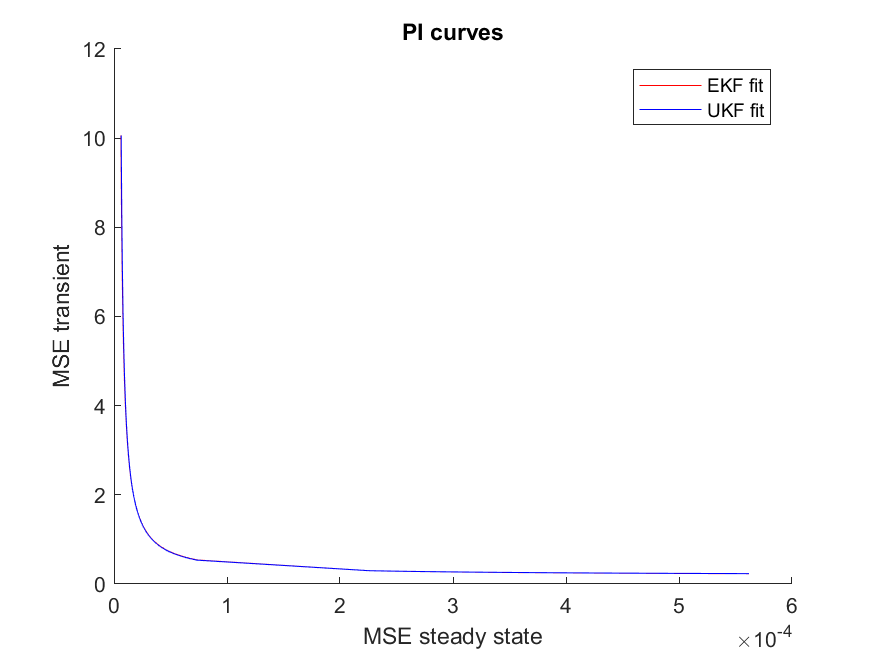
\includegraphics[width=\textwidth]{{images/results/pi/pi_fit_sn_0.005_sno0.000_q1.00e-06}.png}
            \caption{Our results. These have been obtained by a Least Square fit of a generic hyperbola $a+\frac{b}{x+c}$ over the raw data shown in Table~\ref{tab:pi_results}, $q=\num{1e-6}$, SNR 46 \si{\decibel}. $MSE_{\text{fit}} = \num{6.3e-3}$ }
            \label{fig:pi_fit}
        \end{subfigure}
        \begin{subfigure}{0.8\textwidth}
            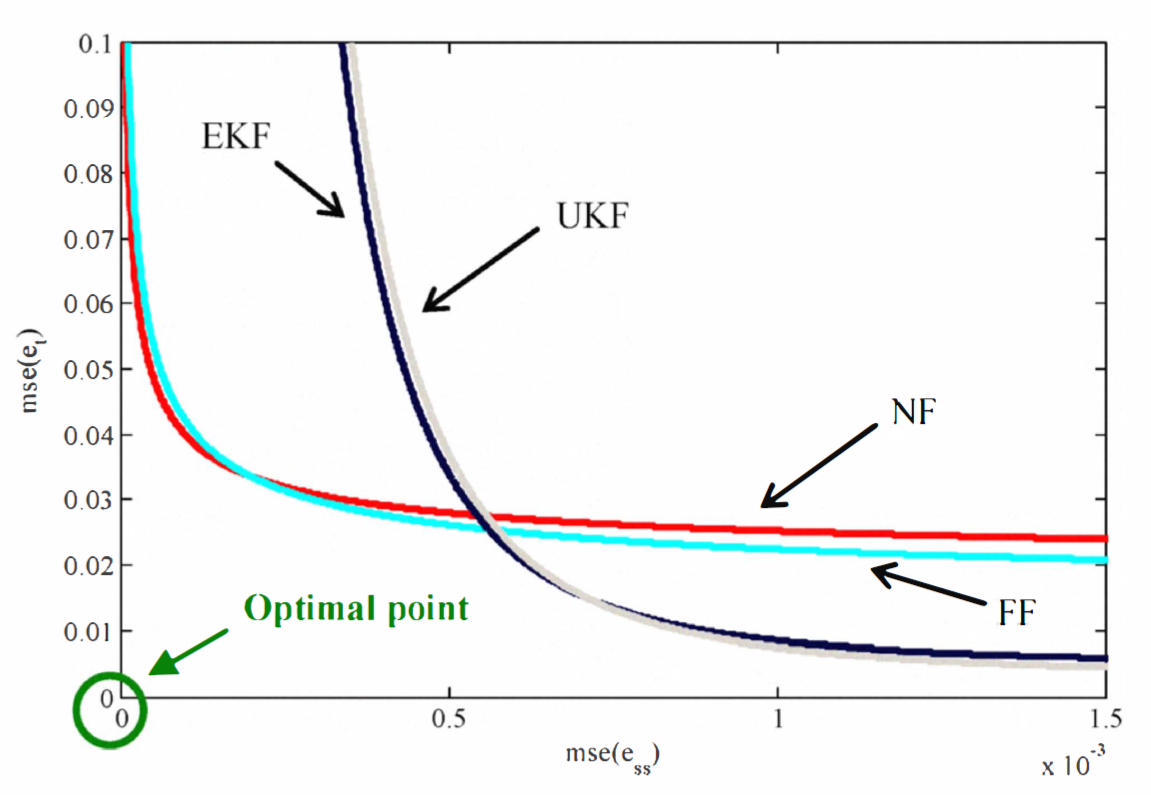
\includegraphics[width=\textwidth]{images/from_paper/pi_curves.png}
            \caption{Results from \cite[Figure~3]{UKF}}
        \end{subfigure}
        }
    \caption{PI curves comparison}
    \label{fig:results_comparison}
\end{figure}
\newcommand{\pifigurewidth}{0.29}

\begin{table}
    \makebox[\linewidth][c]{
    \centering
    \begin{tabular}{|c|cccc|}
        \hline
        & \multicolumn{4}{c|}{SNR}\\
        \cline{2-5}
        q & $\infty$ & $46 \si{\decibel}$ & $22 \si{\decibel}$ & $15 \si{\decibel}$\\
        \hline
        \num{1e-3} & 
        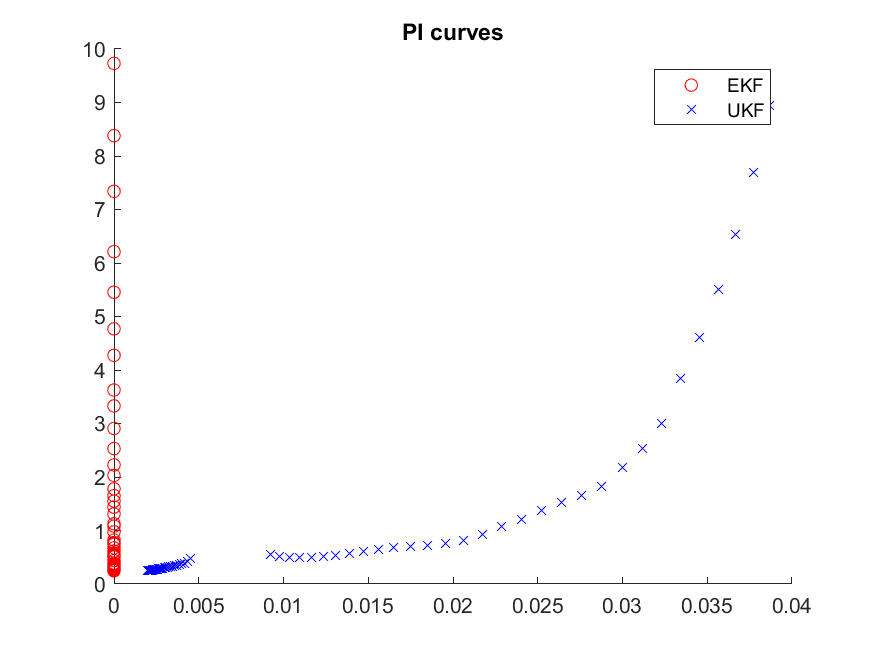
\includegraphics[width=\pifigurewidth\linewidth,align=c]{{images/results/pi/sigma_curves/pi_cloud_sn_0.000_sno0.000_q1.00e-03}.png} &
        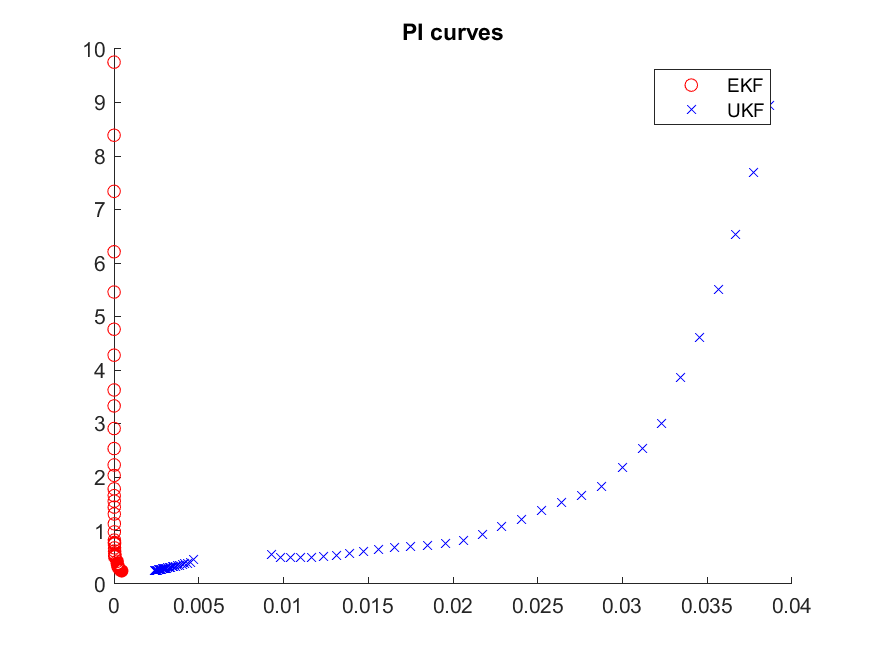
\includegraphics[width=\pifigurewidth\linewidth,align=c]{{images/results/pi/sigma_curves/pi_cloud_sn_0.005_sno0.000_q1.00e-03}.png} &
        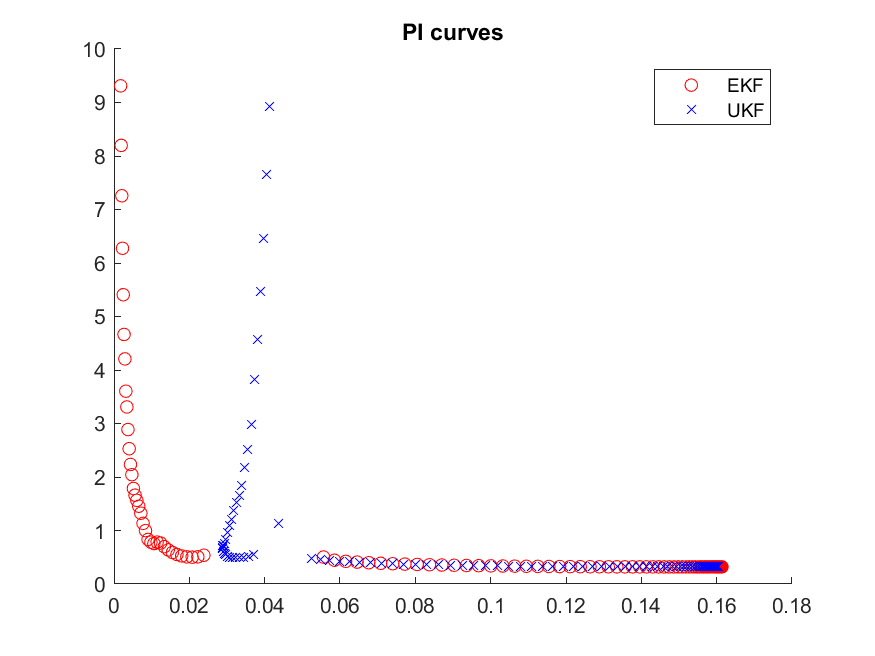
\includegraphics[width=\pifigurewidth\linewidth,align=c]{{images/results/pi/sigma_curves/pi_cloud_sn_0.080_sno0.000_q1.00e-03}.png} &
        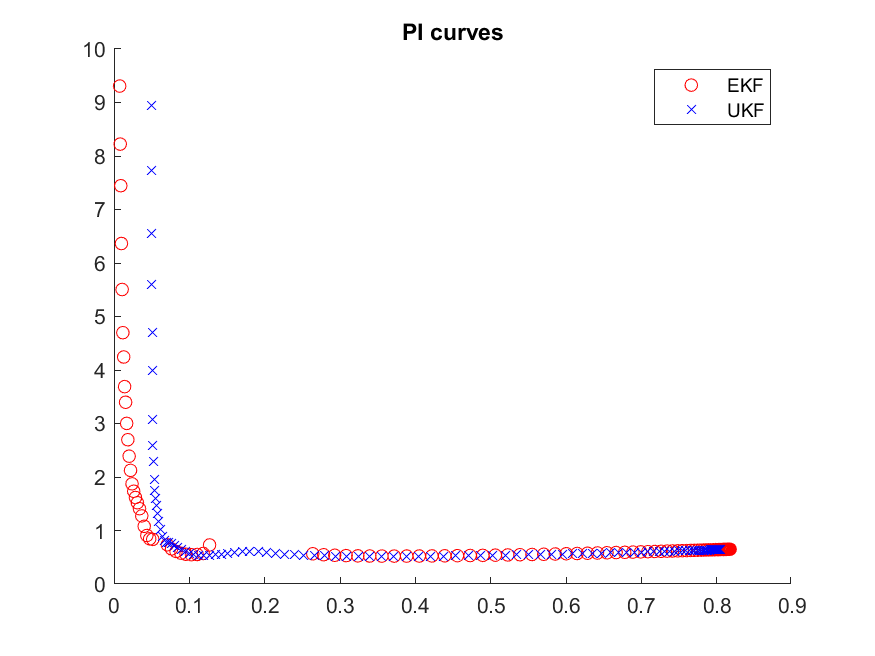
\includegraphics[width=\pifigurewidth\linewidth,align=c]{{images/results/pi/sigma_curves/pi_cloud_sn_0.170_sno0.000_q1.00e-03}.png}\\
        \num{1e-4} & 
        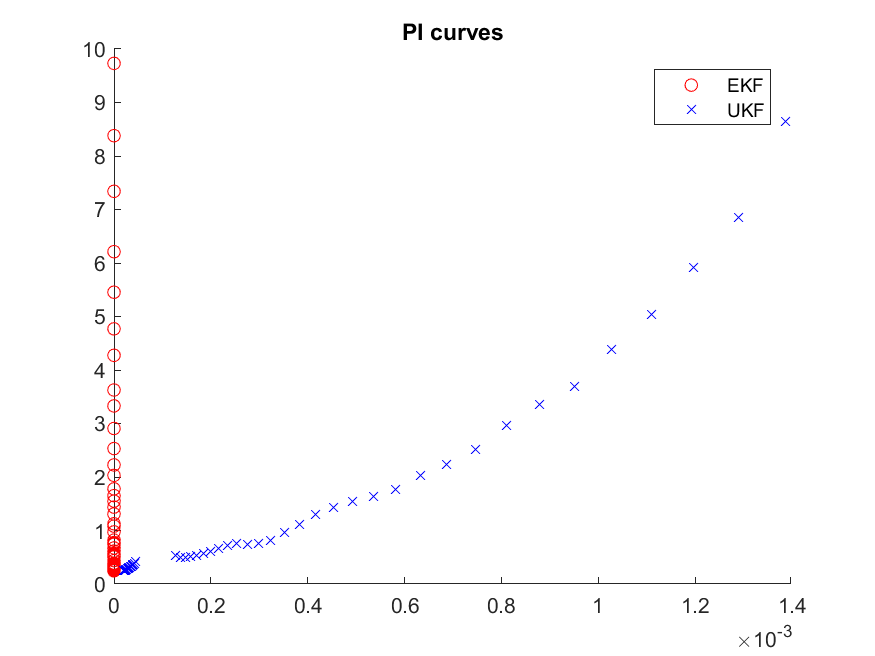
\includegraphics[width=\pifigurewidth\linewidth,align=c]{{images/results/pi/sigma_curves/pi_cloud_sn_0.000_sno0.000_q1.00e-04}.png} &
        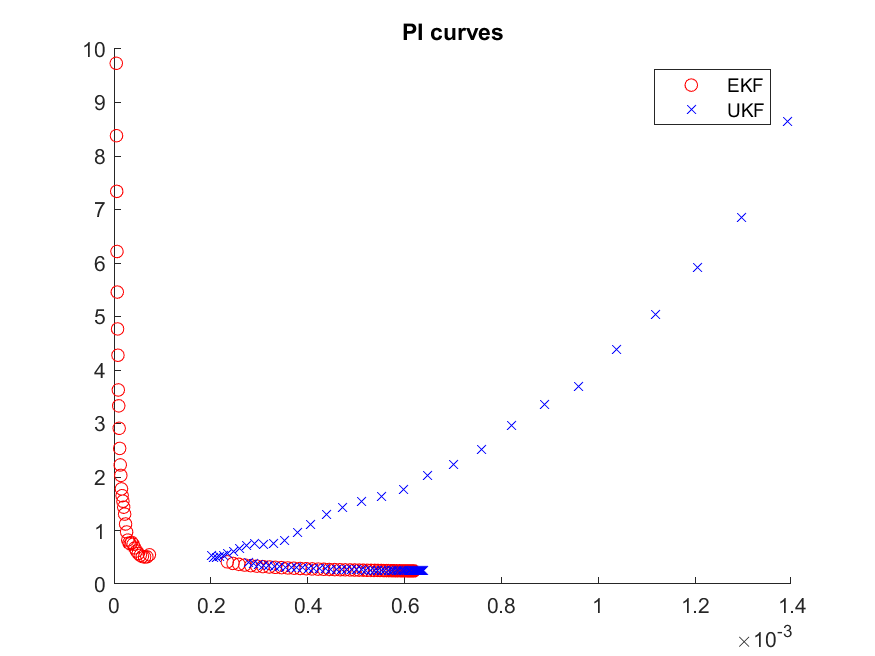
\includegraphics[width=\pifigurewidth\linewidth,align=c]{{images/results/pi/sigma_curves/pi_cloud_sn_0.005_sno0.000_q1.00e-04}.png} &
        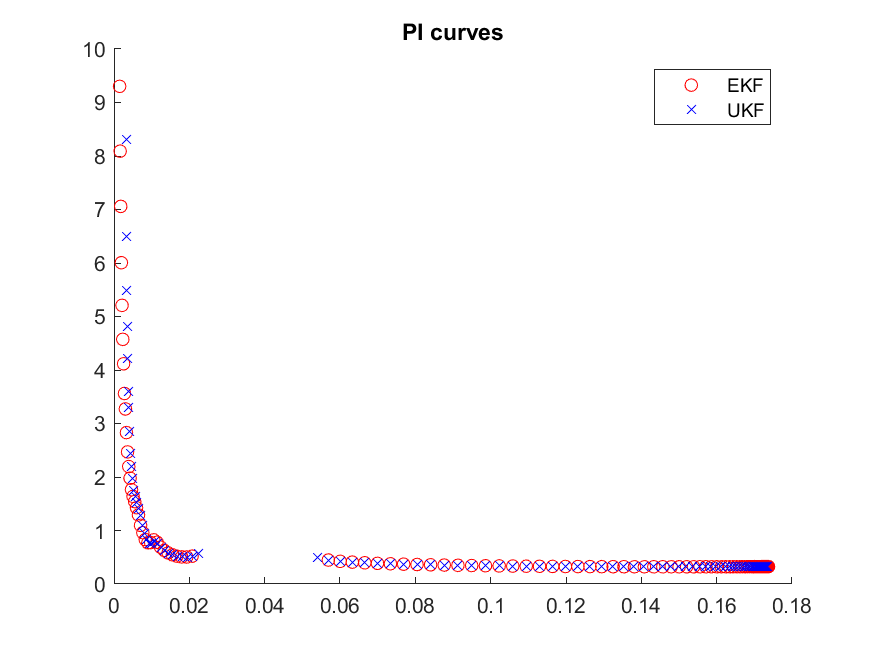
\includegraphics[width=\pifigurewidth\linewidth,align=c]{{images/results/pi/sigma_curves/pi_cloud_sn_0.080_sno0.000_q1.00e-04}.png} &
        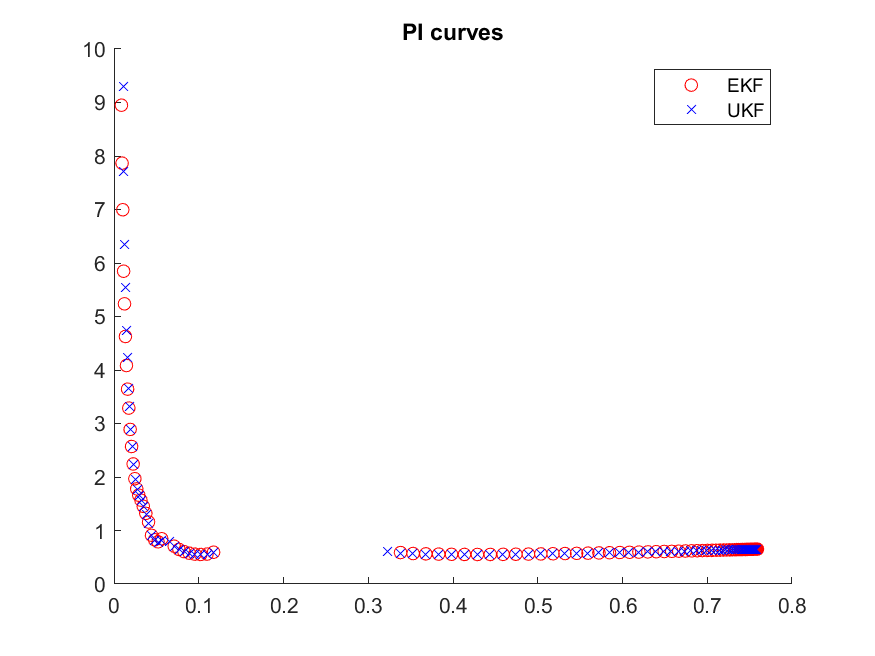
\includegraphics[width=\pifigurewidth\linewidth,align=c]{{images/results/pi/sigma_curves/pi_cloud_sn_0.170_sno0.000_q1.00e-04}.png}\\
        \num{1e-5} & 
        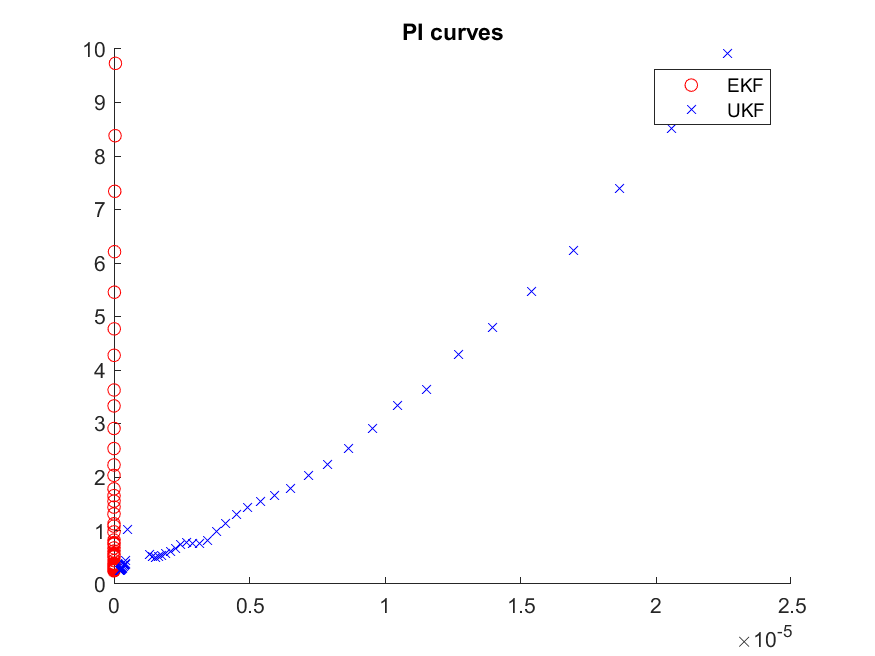
\includegraphics[width=\pifigurewidth\linewidth,align=c]{{images/results/pi/sigma_curves/pi_cloud_sn_0.000_sno0.000_q1.00e-05}.png} &
        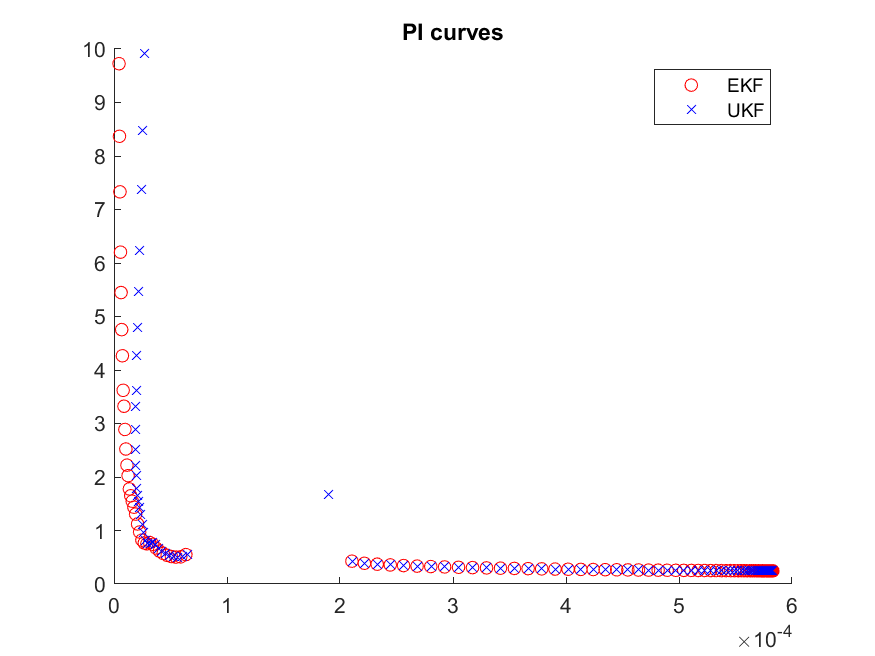
\includegraphics[width=\pifigurewidth\linewidth,align=c]{{images/results/pi/sigma_curves/pi_cloud_sn_0.005_sno0.000_q1.00e-05}.png} &
        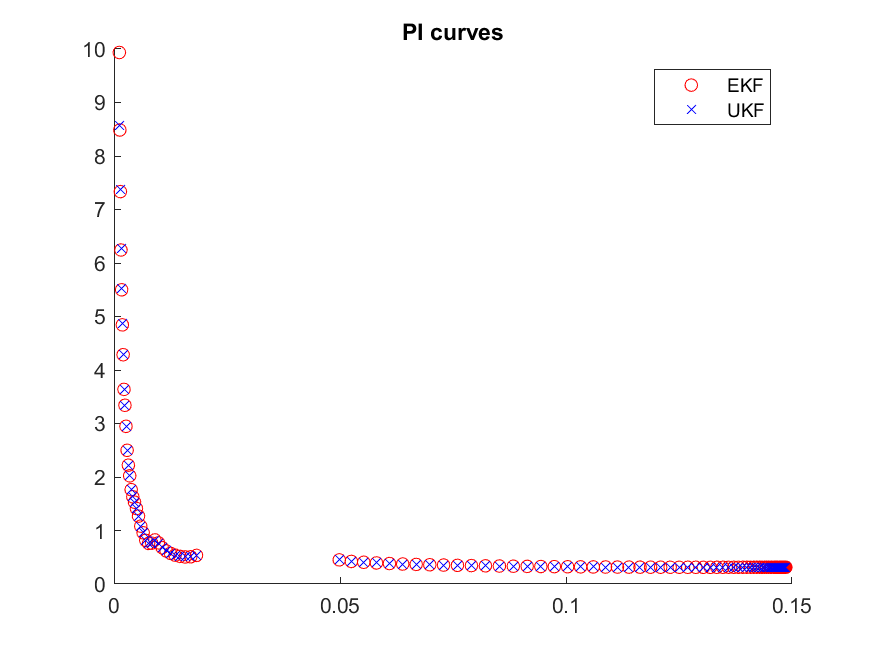
\includegraphics[width=\pifigurewidth\linewidth,align=c]{{images/results/pi/sigma_curves/pi_cloud_sn_0.080_sno0.000_q1.00e-05}.png} &
        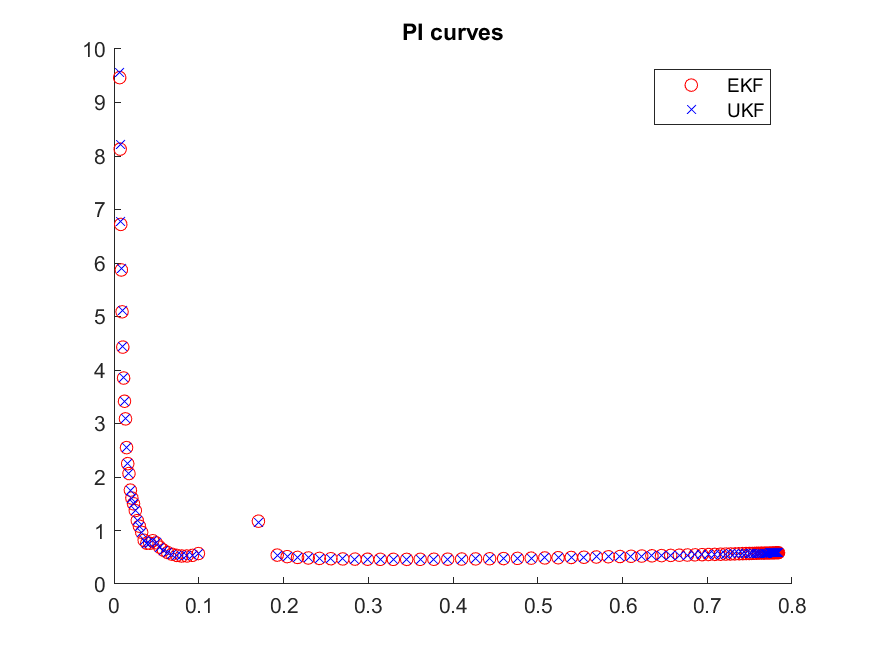
\includegraphics[width=\pifigurewidth\linewidth,align=c]{{images/results/pi/sigma_curves/pi_cloud_sn_0.170_sno0.000_q1.00e-05}.png}\\
        \num{1e-6} & 
        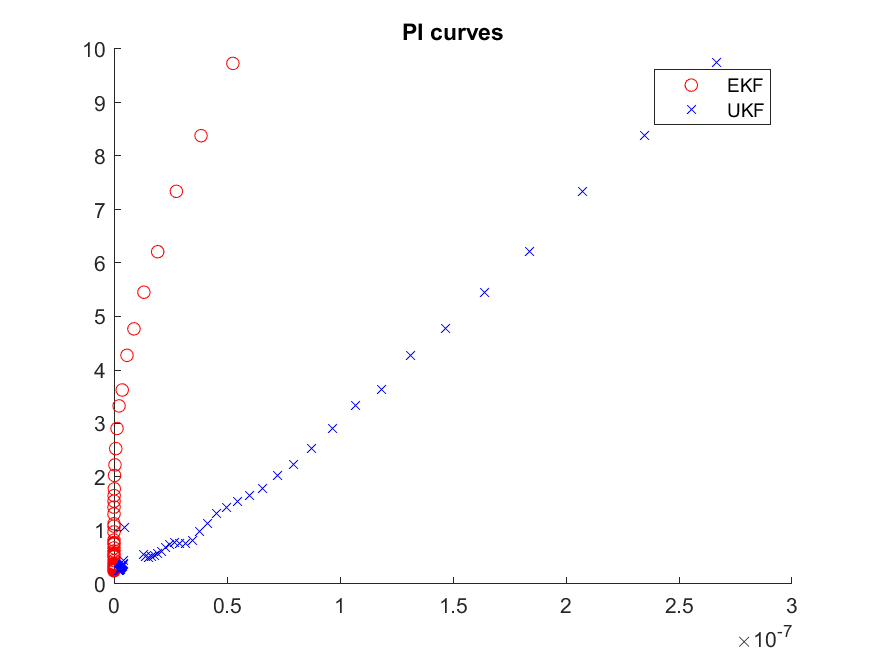
\includegraphics[width=\pifigurewidth\linewidth,align=c]{{images/results/pi/sigma_curves/pi_cloud_sn_0.000_sno0.000_q1.00e-06}.png} &
        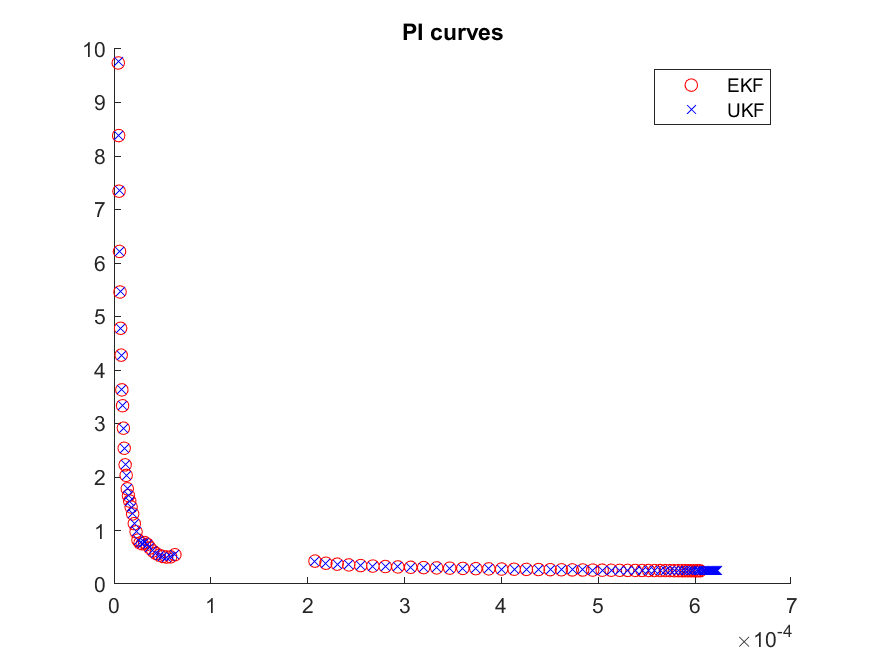
\includegraphics[width=\pifigurewidth\linewidth,align=c]{{images/results/pi/sigma_curves/pi_cloud_sn_0.005_sno0.000_q1.00e-06}.png} &
        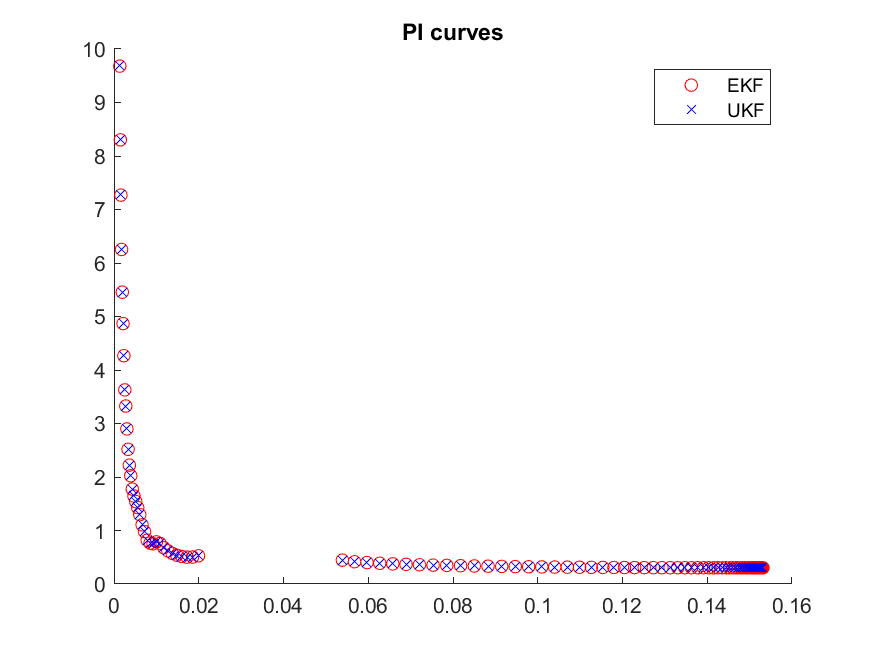
\includegraphics[width=\pifigurewidth\linewidth,align=c]{{images/results/pi/sigma_curves/pi_cloud_sn_0.080_sno0.000_q1.00e-06}.png} &
        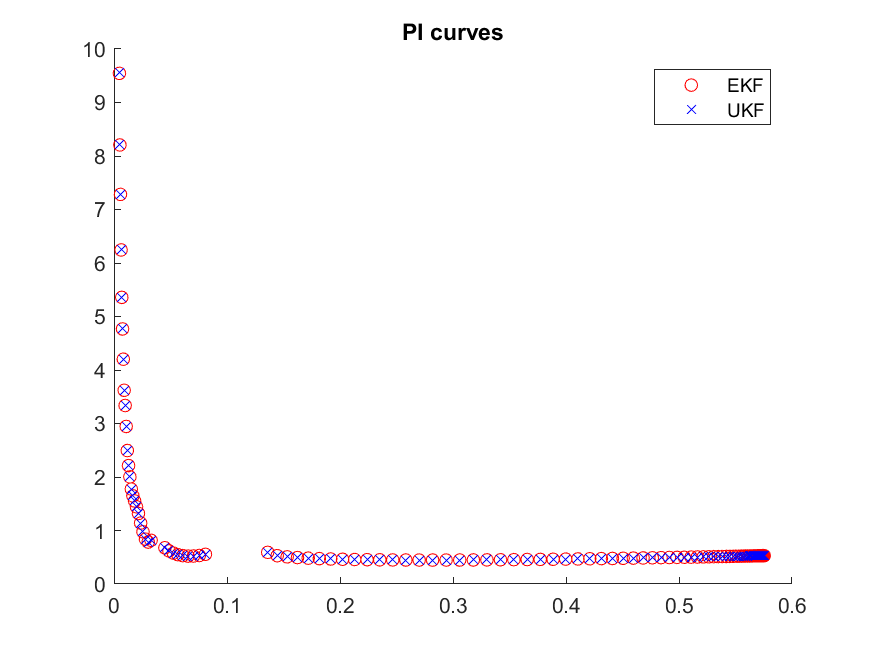
\includegraphics[width=\pifigurewidth\linewidth,align=c]{{images/results/pi/sigma_curves/pi_cloud_sn_0.170_sno0.000_q1.00e-06}.png}\\
        \num{1e-7} & 
        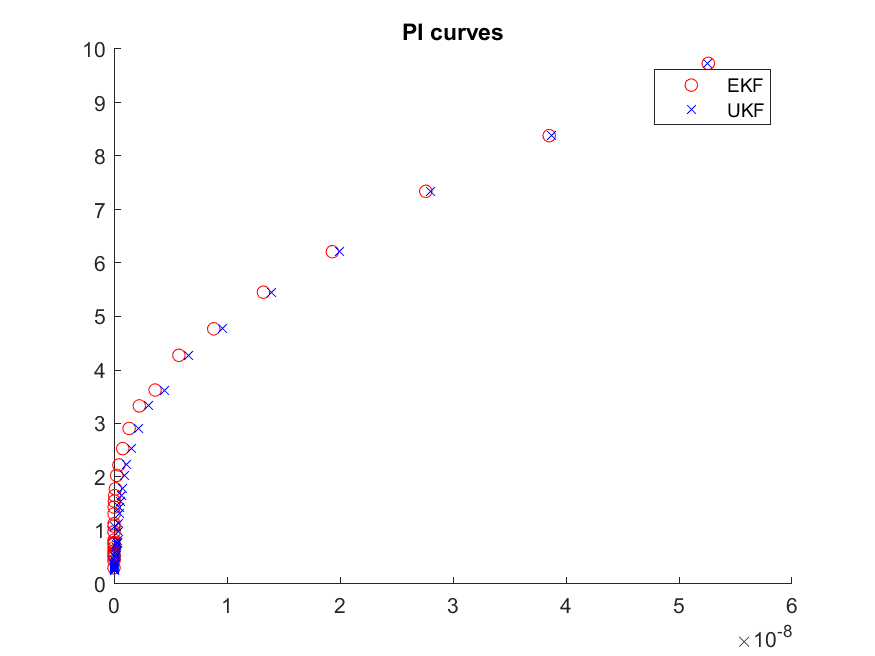
\includegraphics[width=\pifigurewidth\linewidth,align=c]{{images/results/pi/sigma_curves/pi_cloud_sn_0.000_sno0.000_q1.00e-07}.png} &
        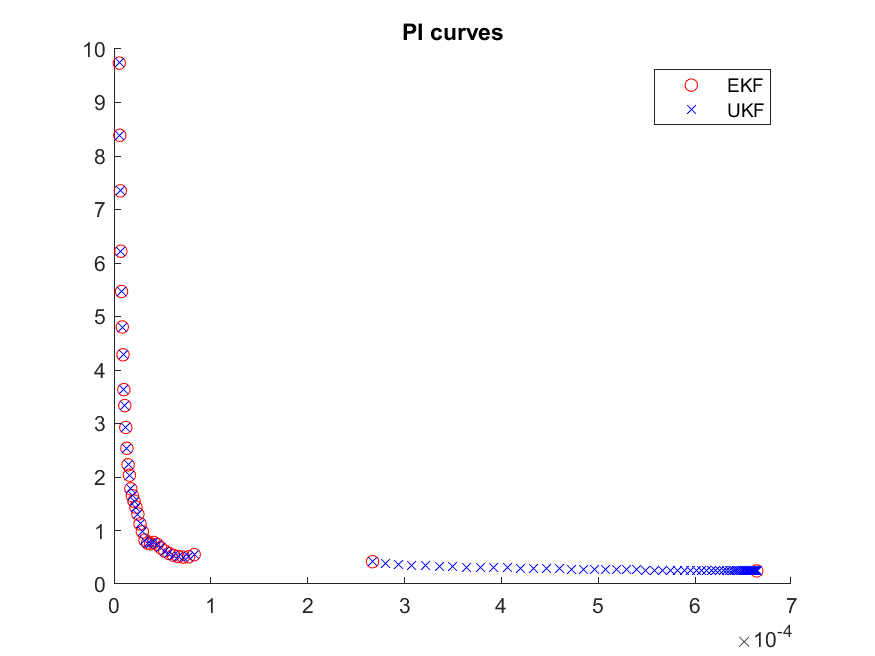
\includegraphics[width=\pifigurewidth\linewidth,align=c]{{images/results/pi/sigma_curves/pi_cloud_sn_0.005_sno0.000_q1.00e-07}.png} &
        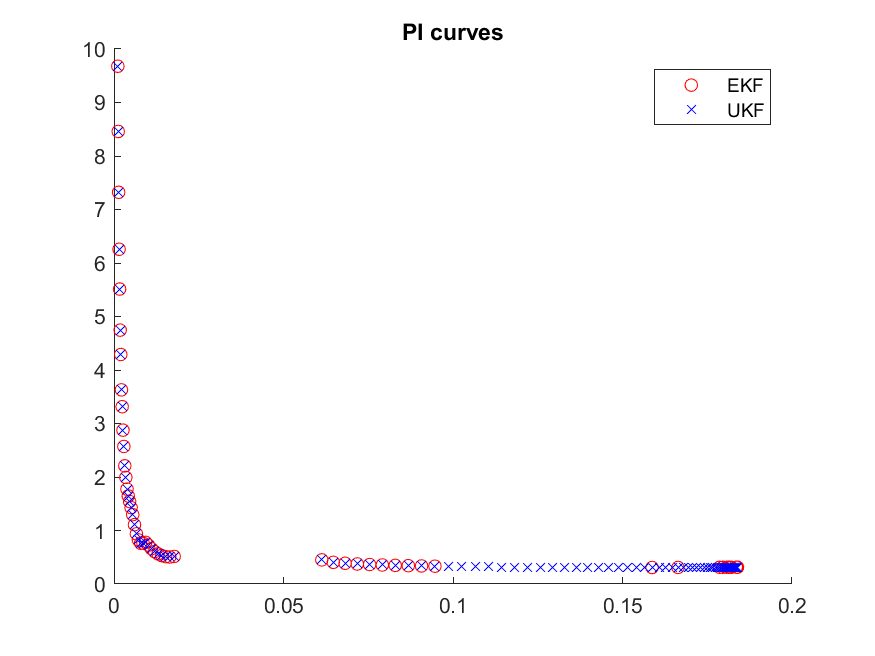
\includegraphics[width=\pifigurewidth\linewidth,align=c]{{images/results/pi/sigma_curves/pi_cloud_sn_0.080_sno0.000_q1.00e-07}.png} &
        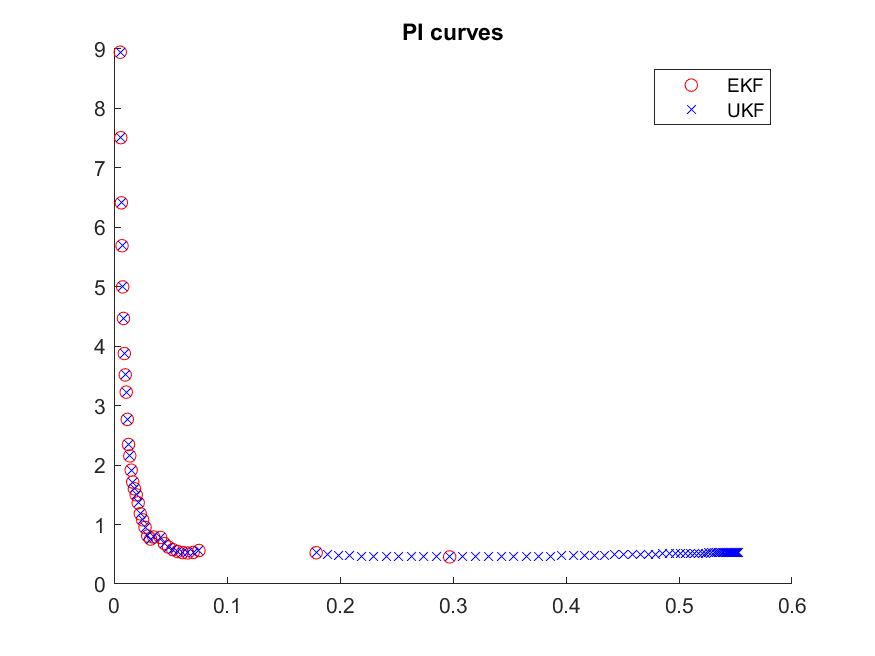
\includegraphics[width=\pifigurewidth\linewidth,align=c]{{images/results/pi/sigma_curves/pi_cloud_sn_0.170_sno0.000_q1.00e-07}.png}\\
        \num{1e-8} & 
        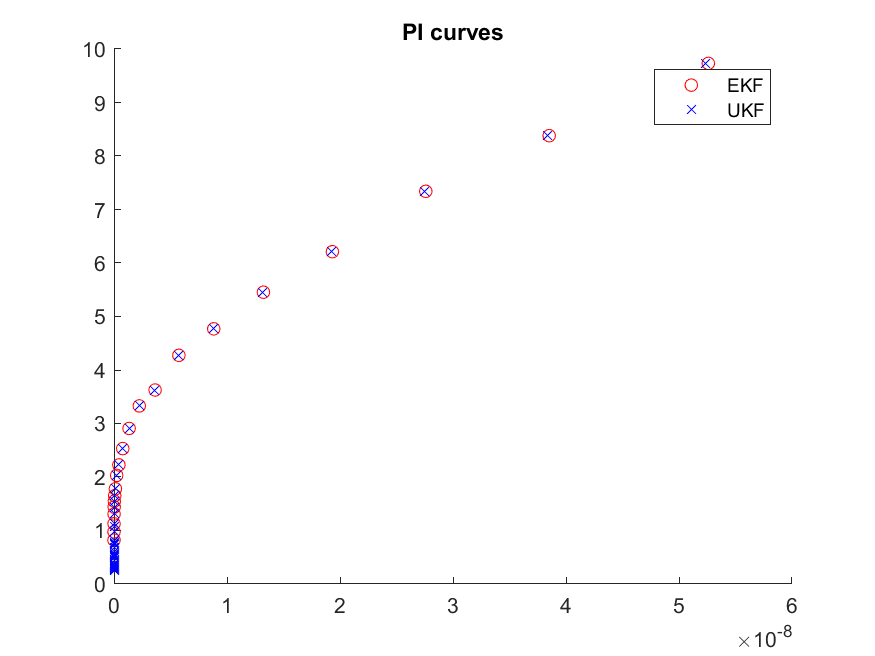
\includegraphics[width=\pifigurewidth\linewidth,align=c]{{images/results/pi/sigma_curves/pi_cloud_sn_0.000_sno0.000_q1.00e-08}.png} &
        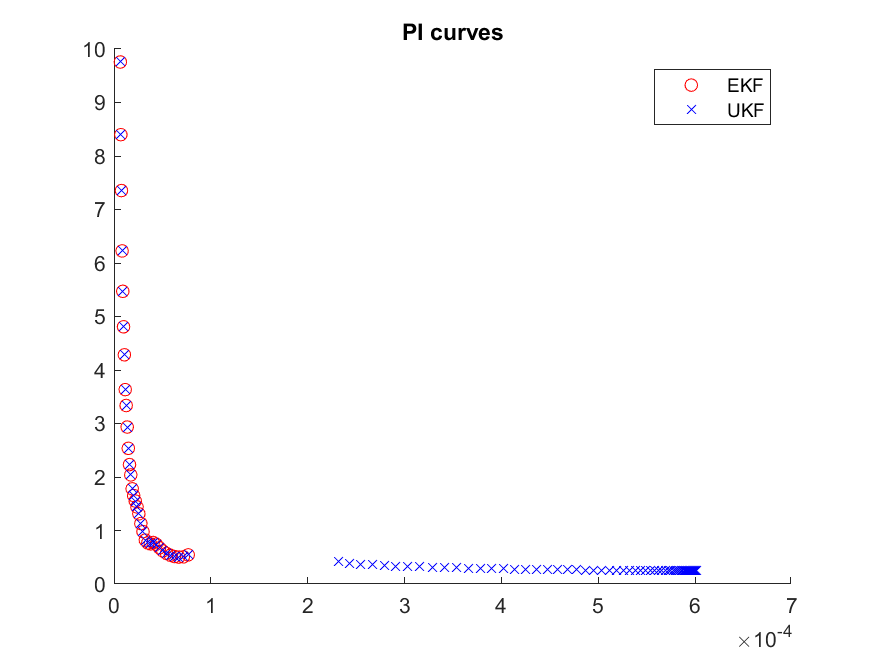
\includegraphics[width=\pifigurewidth\linewidth,align=c]{{images/results/pi/sigma_curves/pi_cloud_sn_0.005_sno0.000_q1.00e-08}.png} &
        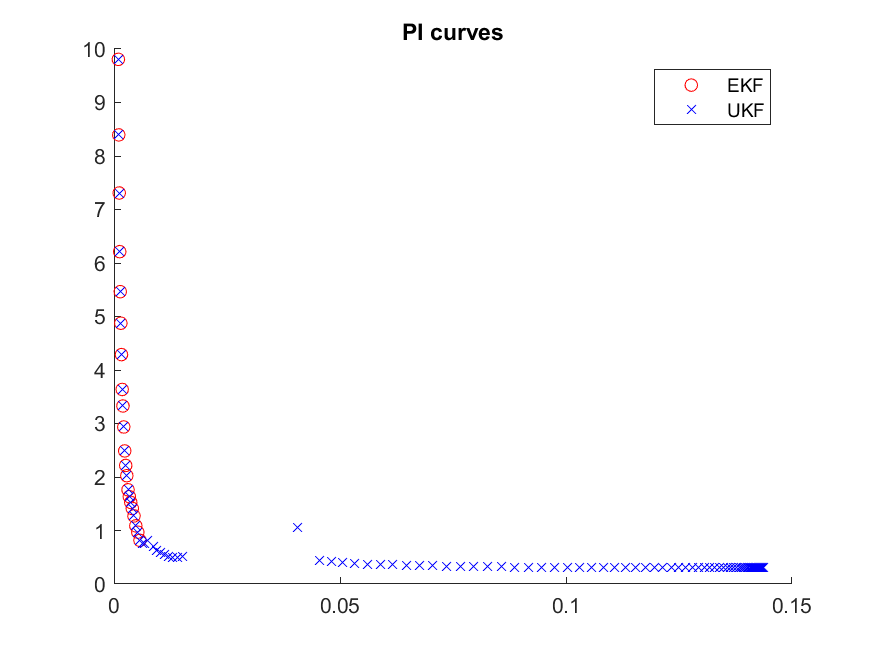
\includegraphics[width=\pifigurewidth\linewidth,align=c]{{images/results/pi/sigma_curves/pi_cloud_sn_0.080_sno0.000_q1.00e-08}.png} &
        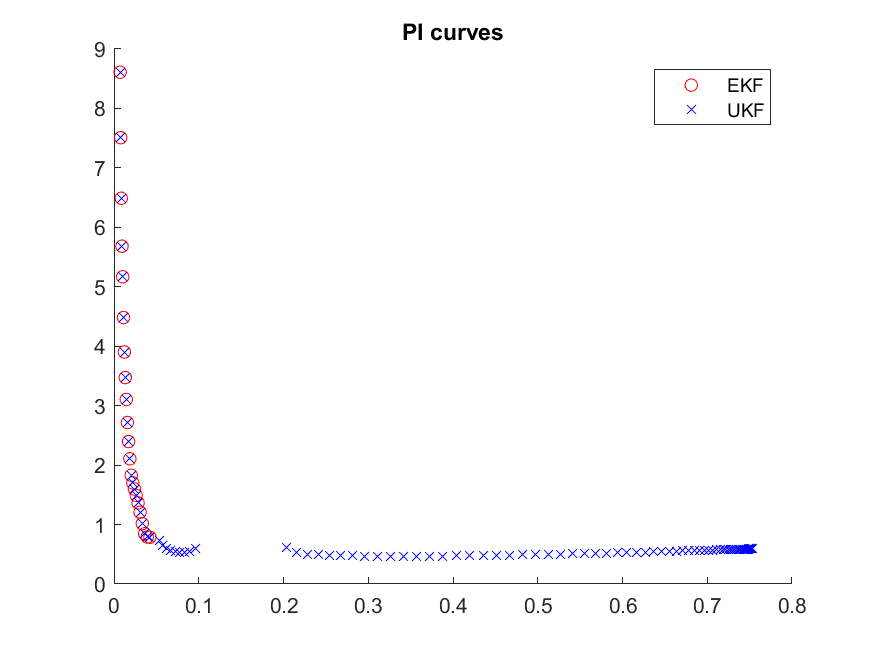
\includegraphics[width=\pifigurewidth\linewidth,align=c]{{images/results/pi/sigma_curves/pi_cloud_sn_0.170_sno0.000_q1.00e-08}.png}\\
        \hline
    \end{tabular}
    }
    \caption{Obtained curves for the PI. On the $x$ axis is the $e_{ss}$, while on the $y$ axis is the $e_t$. Thresholding has been applied to remove non converged iterations.}
    \label{tab:pi_results}
\end{table}
\begin{figure}
    \centering
    \captionsetup{width=.8\textwidth}
    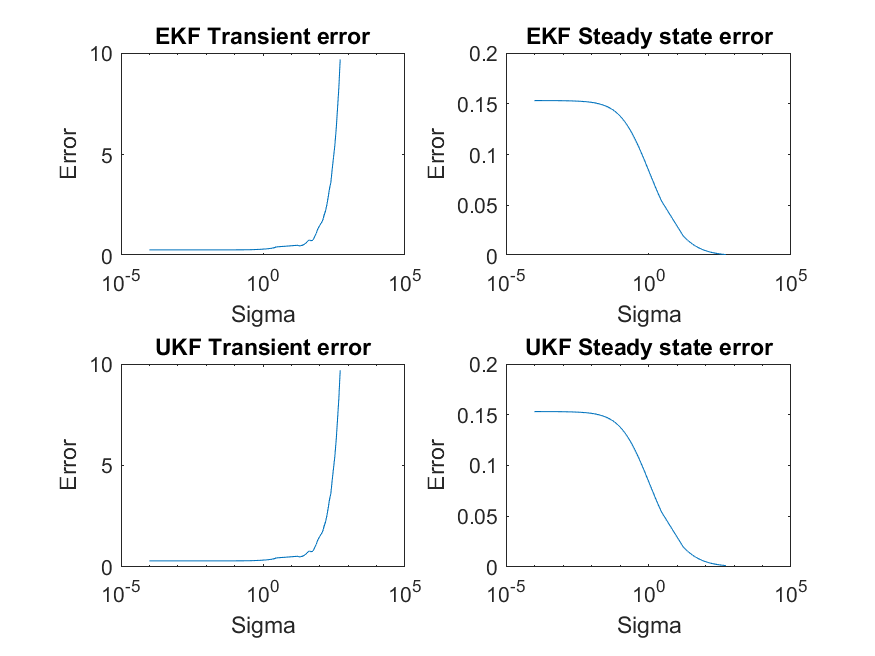
\includegraphics[width=0.8\textwidth]{{images/results/pi/error_curves/sigma_error_figure_sn_0.080_sno0.000_q1.00e-06}.png}
    \caption{The error as a function of $\sigma$ (SNR 22 \si{\decibel}). It is evident that $\sigma$ regulates the tradeoff between convergence speed and quality.}
    \label{fig:sigma_error}
\end{figure}
\begin{figure}
\makebox[\linewidth][c]{
    \centering
    \begin{subfigure}{0.45\textwidth}
    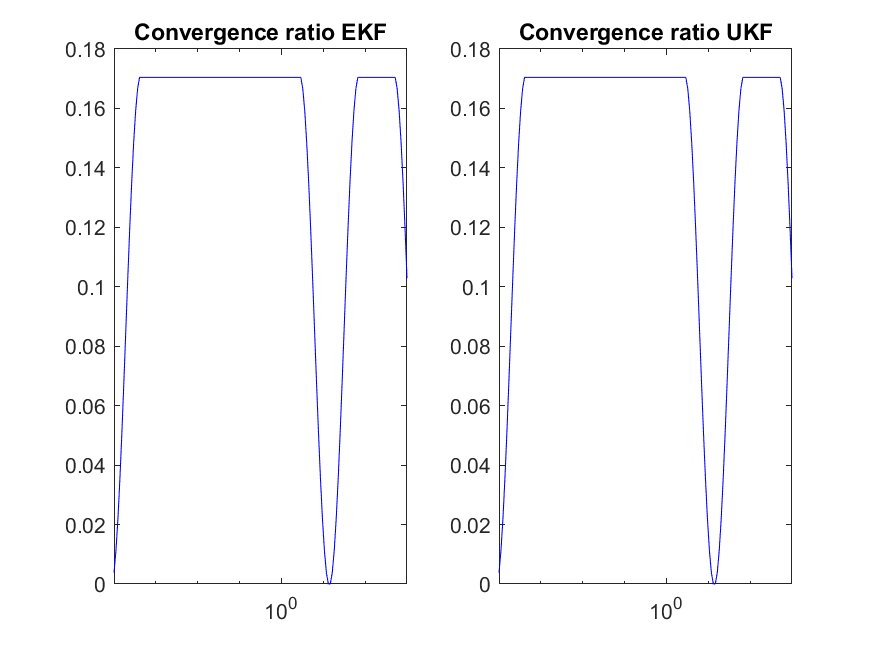
\includegraphics[width=\textwidth]{{images/results/pi/convergence_ratio_curves/convergence_sn_0.080_sno0.000_q1.00e-06}.png}
    \caption{$q=\num{1e-6}$}
    \end{subfigure}
    \quad
    \begin{subfigure}{0.45\textwidth}
    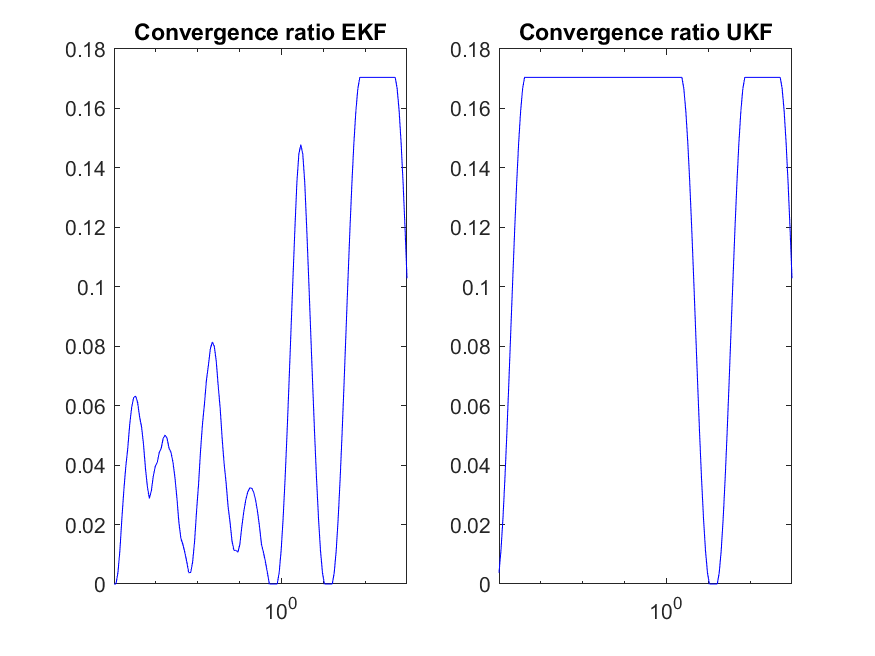
\includegraphics[width=\textwidth]{{images/results/pi/convergence_ratio_curves/convergence_sn_0.080_sno0.000_q1.00e-07}.png}
    \caption{$q=\num{1e-7}$}
    \end{subfigure}
    \quad
    \begin{subfigure}{0.45\textwidth}
    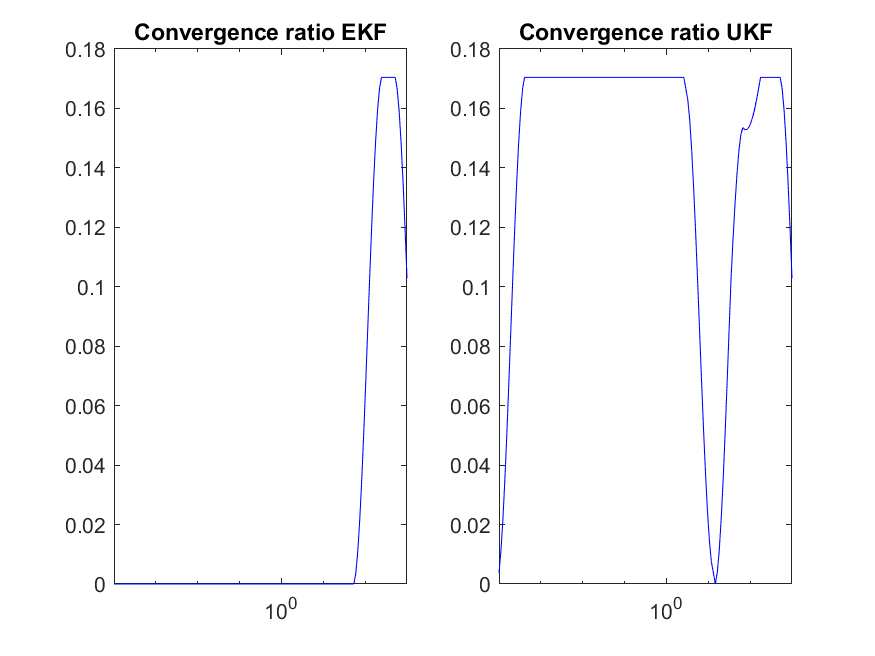
\includegraphics[width=\textwidth]{{images/results/pi/convergence_ratio_curves/convergence_sn_0.080_sno0.000_q1.00e-08}.png}
    \caption{$q=\num{1e-8}$}
    \end{subfigure}
}
\caption{Convergence ratios as a function of $\sigma$ (22 \si{\decibel})}
\label{fig:convergence_ratio}
\end{figure}
In this section the results obtained from the experiments are discussed.

\subsection{PI}
In Figure~\ref{fig:results_comparison} the smoothest fit for the PI curve is shown. It is really similar to \cite[Figure~3]{UKF}. The original noise profile and the original parameters are unknown; our best $e_t$ is one orders of magnitude bigger than the best one by \citeauthor{UKF} (\num{2.5e-1}), but we are able to obtain a steady state error of \num{3.28e-6}, two orders of magnitude smaller. With no noise, the best performances for both EKF and UKF are of the order of $e_{ss} \sim 10^{-26}$.

In Table~\ref{tab:pi_results} we see the effects of $q$. These may be due to finite arithmetic precision. In the lower-right portion of the image, the shape of the curve is more or less invariant, even in high noise conditions; however, the EKF stops converging at really small $q$s and small $\sigma$s (absence of red points). This is highlighted also in Figure~\ref{fig:convergence_ratio}. We can observe that in the Riccati equation, the matrix $HPH^T +q$ is inverted. With low noise and low $q$, both terms are really small ($\sim10^{-8}$ before diverging), pointing to a possible numerical error.

We can also see how, for big $q$s and big $\sigma$s, the UKF changes behavior abruptly as $r$ grows, (e.g., in Figure~\ref{tab:pi_results}, q = \num{1e-3}, 22 \si{\decibel}, or q = \num{1e-4} 46 \si{\decibel}), without compromising on convergence ratios, and mantaining comparable performances with the EKF. Since $r$ is summed to the propagated sigma points, having an $r$ 3-7 orders of magnitude bigger than the terms of $\mathrm{Cov}(\varsigma^s_k,\varsigma^m_k)$ and $\mathrm{Cov}(\varsigma^m_k,\varsigma^m_k)$ may be the source of the weird behavior, given the variable resolution of the floating point representation.

There is also a valley in the convergence ratio with $15 \leq \sigma \leq 30$ for both algorithms, which we were not able to explain.

\subsection{RI}
\begin{figure}
\centering
\begin{subfigure}{0.45\textwidth}
\includemedia[width=\textwidth,activate=onclick,addresource=images/animations/ri_lownoise.mp4,flashvars={source=images/animations/ri_lownoise.mp4&loop=true&autoPlay=true}]{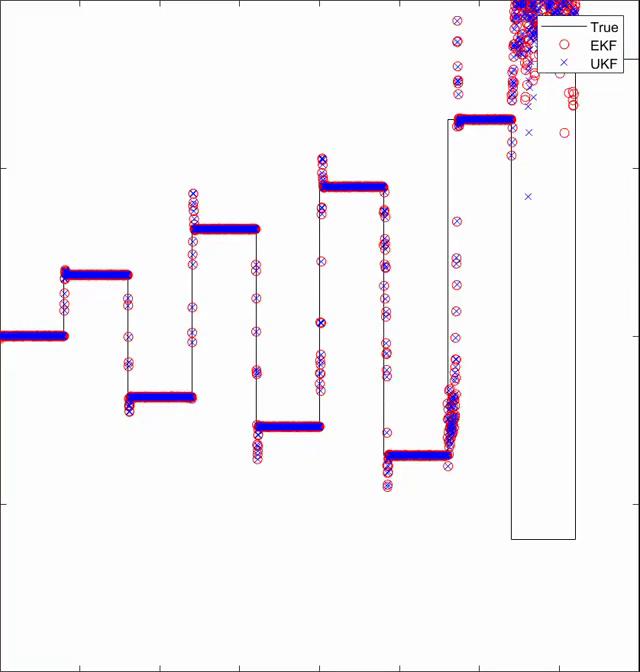
\includegraphics[width=\textwidth]{images/animations/ri_lownoise_thumb.png}}{VPlayer.swf}
\caption{SNR $34\si{\decibel}$, $\sigma_{\omega,\text{noise}}=0$}
\label{fig:ri_lownoise_anim}
\end{subfigure}
\quad
\begin{subfigure}{0.45\textwidth}
\includemedia[
width=\textwidth,activate=onclick,addresource=images/animations/ri_highnoise.mp4,flashvars={
source=images/animations/ri_highnoise.mp4&loop=true&autoPlay=true}]{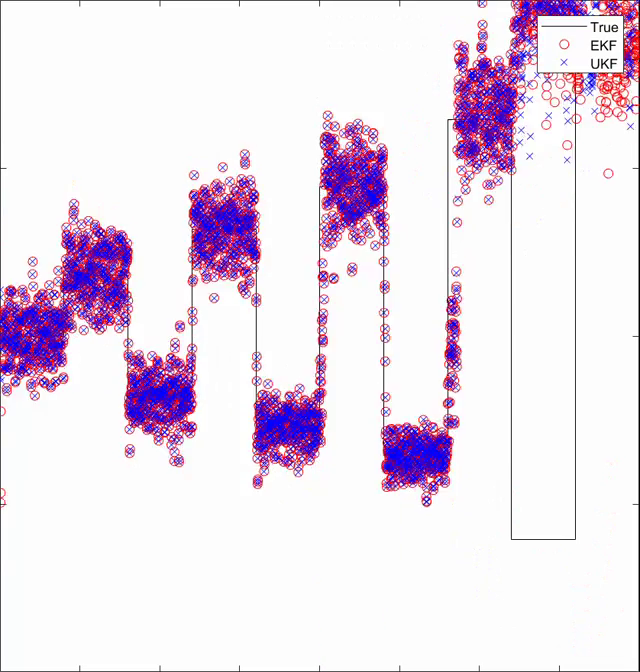
\includegraphics[width=\textwidth]{images/animations/ri_highnoise_thumb.png}}{VPlayer.swf}
\caption{SNR $8\si{\decibel}$, $\sigma_{\omega,\text{noise}}=30\%$}
\label{fig:ri_highnoise_anim}
\end{subfigure}

\caption{Visualization of some predictions for the computation of the RI index with $\sigma=\num{1e+1}$, $q=\num{1e-5}$}
\label{fig:ri_animation}
\end{figure}
\begin{figure}
    \makebox[\linewidth][c]{
        \centering
        \begin{subfigure}{0.45\textwidth}
        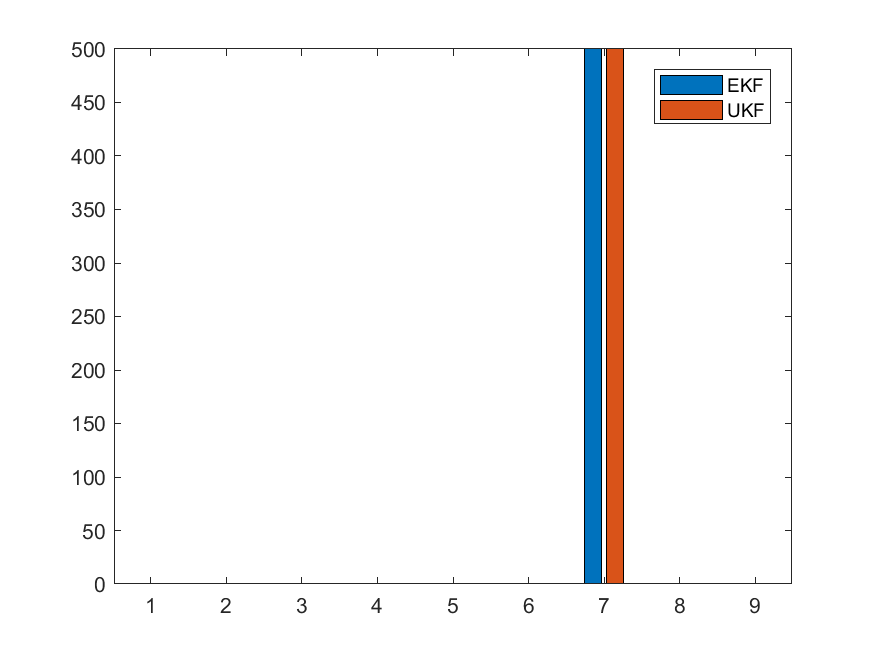
\includegraphics[width=\textwidth]{{images/results/ri/ri_figure_q1.00e-05_s1.00e+01_sn2.00e-02_sno1.00e-03}.png}
        \caption{Results for test in \ref{fig:ri_lownoise_anim}}
        \label{fig:ri_lownoise}
        \end{subfigure}
        \quad
        \begin{subfigure}{0.45\textwidth}
        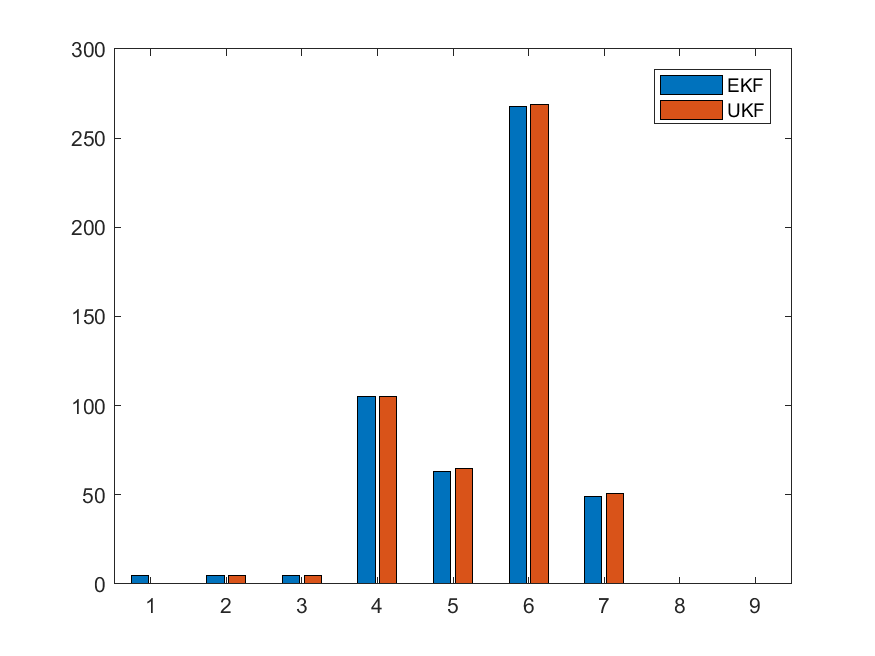
\includegraphics[width=\textwidth]{{images/results/ri/ri_figure_q1.00e-05_s1.00e+01_sn4.00e-01_sno3.00e-01}.png}
        \caption{Results for test in \ref{fig:ri_highnoise_anim}}
        \label{fig:ri_highnoise}
        \end{subfigure}
        \quad
        \begin{subfigure}{0.45\textwidth}
        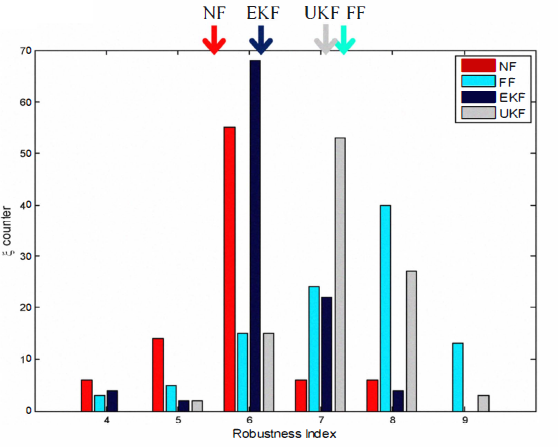
\includegraphics[width=\textwidth]{images/from_paper/ri_paper.png}
        \caption{Results shown in \cite[Figure~6]{UKF}}
        \label{fig:ri_paper}
        \end{subfigure}
    }
    \caption{Results for simulations shown in Figure~\ref{fig:ri_animation}, 500 iterations}
    \label{fig:ri_results}
\end{figure}
Multiple simulations have been performed with several parameter combinations. In Figure~\ref{fig:ri_animation} two visualizations of the prediction are shown for the two algorithms with two different SNRs. In Figure~\ref{fig:ri_results} are the results obtained. With low noise the algorithm always converged until step 7, then getting stuck at $\pi$ (Figure~\ref{fig:ri_lownoise}). With high noise, although the performance are worsened, we see that the algorithm is sometimes able to converge at step 8. 

\medskip
 
\printbibliography

\end{document}
